\section{Use Cases}

Si sono presi in considerazione i seguenti casi d'uso, ossia quelli a priorità più elevata della Tabella~\ref{tab:use_cases_high_priority}

\begin{table}[htbp]
	\centering
	\begin{tabularx}{\textwidth}{|>{\centering\arraybackslash} m{4em}| >{\raggedright\arraybackslash}X |}
		\hline
		\textbf{Codice} & \textbf{Titolo} \\ [0.5ex]
		\hline\hline
		UC1 & Gestione comanda  \\
		\hline
		UC2 & Effettuare un'ordinazione \\
		\hline
		UC3 & Visualizzare menù \\
		\hline
		UC4 & Autenticazione \\
		\hline
		UC5 & Visualizzare lista ordini \\
		\hline
		UC6 & Gestione preparazione ordini \\
		\hline
	\end{tabularx}
	\caption{Casi d'uso presi in considerazione nell'iterazione 1}
	\label{tab:use_cases_it1}
\end{table}

\begin{figure}[htbp]
	\centering
	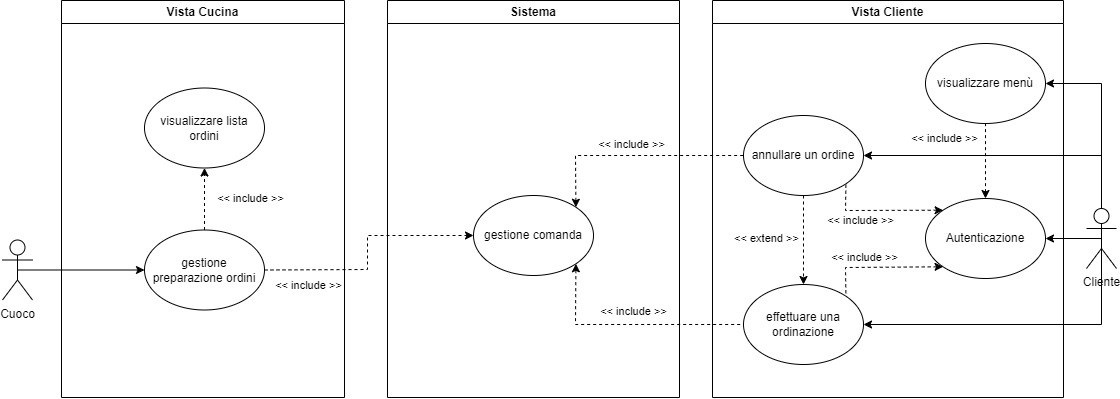
\includegraphics[scale=0.36]{iterazione1/images/useCases_it1.jpg}
	\caption{Casi d'uso presi in considerazione nell'iterazione 1\label{fig:use_cases_it1}}
\end{figure}

Per facilitare una migliore organizzazione e comprensione del sistema, i casi d'uso vengono raggruppati nel seguente modo:

\subsection{Gruppo Sistema}
\paragraph{UC-1 “Gestione Comanda”:}
\begin{itemize}
	\item UC-1.1 : gestione priorità ordine \\ ogni ordine è caratterizzato da una priorità
	\item UC-1.2 : gestione coda ordini \\
	ogni ordine è inserito in una coda ordini
	\item UC-1.3 : assegnazione ordini comanda \\
	ogni ordine deve essere associato ad una comanda
	\item UC-1.4 : assegnazione comanda cliente \\
	ogni comanda deve essere associata ad un cliente
\end{itemize}

\subsection{Gruppo cliente}
\paragraph{UC-2 “effettuare un’ordinazione”:}
\begin{itemize}
	\item UC-2.1 : effettuare un ordine personalizzato \\
	il cliente può effettuare un ordine escludendo un ingrediente o descrivendo una variazione del piatto
\end{itemize}

\paragraph{UC-3 “Visualizzare menu”:}
\begin{itemize}
	\item UC-3.1 : visualizzare piatto 
	\item UC-3.2 : visualizzare informazioni piatto \\
	il cliente deve poter leggere breve descrizione, ingredienti, prezzo
\end{itemize}

\paragraph{UC-4 “Autenticazione”:}
\begin{itemize}
	\item UC-4.1 : identificazione sessione cliente \\ 
	al momento del pasto e solo per il pasto, il cliente deve poter distinguere la propria comanda
\end{itemize}

\subsection{Gruppo cuoco}
\paragraph{UC-5 “visualizzare lista ordini”:}
\begin{itemize}
	\item UC-5.1 : visualizzazione ordini per postazione \\ 
	il cuoco deve visualizzare gli ordini destinati alla sua postazione
\end{itemize}

\paragraph{UC-6 “gestione preparazione ordini”:}
\begin{itemize}
	\item UC-6.1 : notifica preparazione ordine \\ 
	il cuoco deve segnalare la presa in carico dell’ordine
	\item UC-6.2 : notifica completamento ordine \\
	il cuoco deve segnalare il completamento dell’ordine così da passare al successivo
	\item UC-6.3 : gestione priorità postazione \\
	il cuoco può modificare la priorità di un certo ingrediente così da ridurre la pressione su una certa postazione o, viceversa, per aumentarne il traffico. In tal modo può manualmente agire sulla gestione del traffico verso la cucina.
\end{itemize}

\clearpage